\chapter{Graph signal models}
\section{The smoothness assumption}
\label{ch:smoothness}
Going further with the spectral analysis, some other intuitions about the graph spectrum can be conveyed from the classical setting to the graph setting.

One of them is that in the classical setting the eigenvalues carry a specific notion of frequency: complex exponentials related to lower frequencies are relatively smooth, slowly oscillating functions whereas for high frequencies the associated complex exponentials oscillate more rapidly. Reporting this onto the graph spectral settings, we see that the Laplacian eigenfunctions associated with lower eigenvalues can be seen as smooth, while the ones related to higher eigenvalues tend to oscillate more intensively. \cite{Shuman2016} In the specific case of the null eigenvalue  the related eigenvector ($\chi_0$) is constant and equal to $\frac{1}{\sqrt{N}}$ \cite{Shuman2013}.
\subsection{The smoothness in the graph signal domain}
Taking a step back, one of the common simple assumptions about data residing on graphs is that the signal changes smoothly between connected nodes; in this, a simple way to quantify how smooth is a set of vectors residing on a weighted undirected graph is through the function:
\begin{equation}
\frac{1}{2} \sum_{i,j}W_{i,j}||y_i - y_j||^2
\label{eq:smooth}
\end{equation}
with $W_ij$ representing the weight between node $i$ and node $j$, as usual, and $y_i$ and $y_j$ representing two vectors in $y_1, y_2, \dots, y_N \in \R$. This means that if two vectors $y_i$ and $y_j$ reside on two nodes connected by a high $W_{ij}$, then they are expected to have a small distance; on the other hand, if two nodes are considered to have a big distance, then the weight of the edge connecting them should be small.

\subsection{Smoothness in the vertex domain}
The same concept can be translated into the vertex domain under the form:
\begin{equation}
\sum_{i,j}W_{i,j}||\rchi_i - \rchi_j||^2
\label{eq:smoothVertex}
\end{equation}
Where $\rchi_i$ and $\rchi_j$ are the $i^{th}$ and the $j^{th}$ column of the matrix of eigenvectors $\pmb{\rchi}$ related to the graph Laplacian $L$.\\
Rewriting \autoref{eq:smooth} in matrix form, we obtain\cite{Kalofolias2016}:
\begin{equation}
\tr(\rchi^T L \rchi)
\label{eq:smoothMatrix}
\end{equation}
and, recalling that in the Laplacian matrix we can explicit the diagonal matrix containing the associated eigenvalues $\Lambda$:
\begin{equation}
L = \rchi \Lambda \rchi
\label{eq:diag}
\end{equation}
we can thus arrive to the relation between the smoothness and the graph signal spectrum:
\begin{equation}
\tr(\rchi^T L \rchi) = \tr(\rchi^T \rchi \Lambda \rchi^T \rchi) = \tr(\Lambda)
\end{equation}
This result clearly explains the relation between the signal smoothness and the eigenvalues of the Laplacian that we presented at the beginning of the chapter.\autoref{fig:osc} shows different graph Laplacian eigenvectors for a random graph. The eigenvectors associated to larger eigenvalues tend to oscillate more rapidly and to have dissimilar values on vertices connected by a high weight edge, this moreover bringing to higher occurrences of zero crossing associated to the graph Laplacian. \cite{Shuman2013}.

\begin{figure}[tb]
\centering
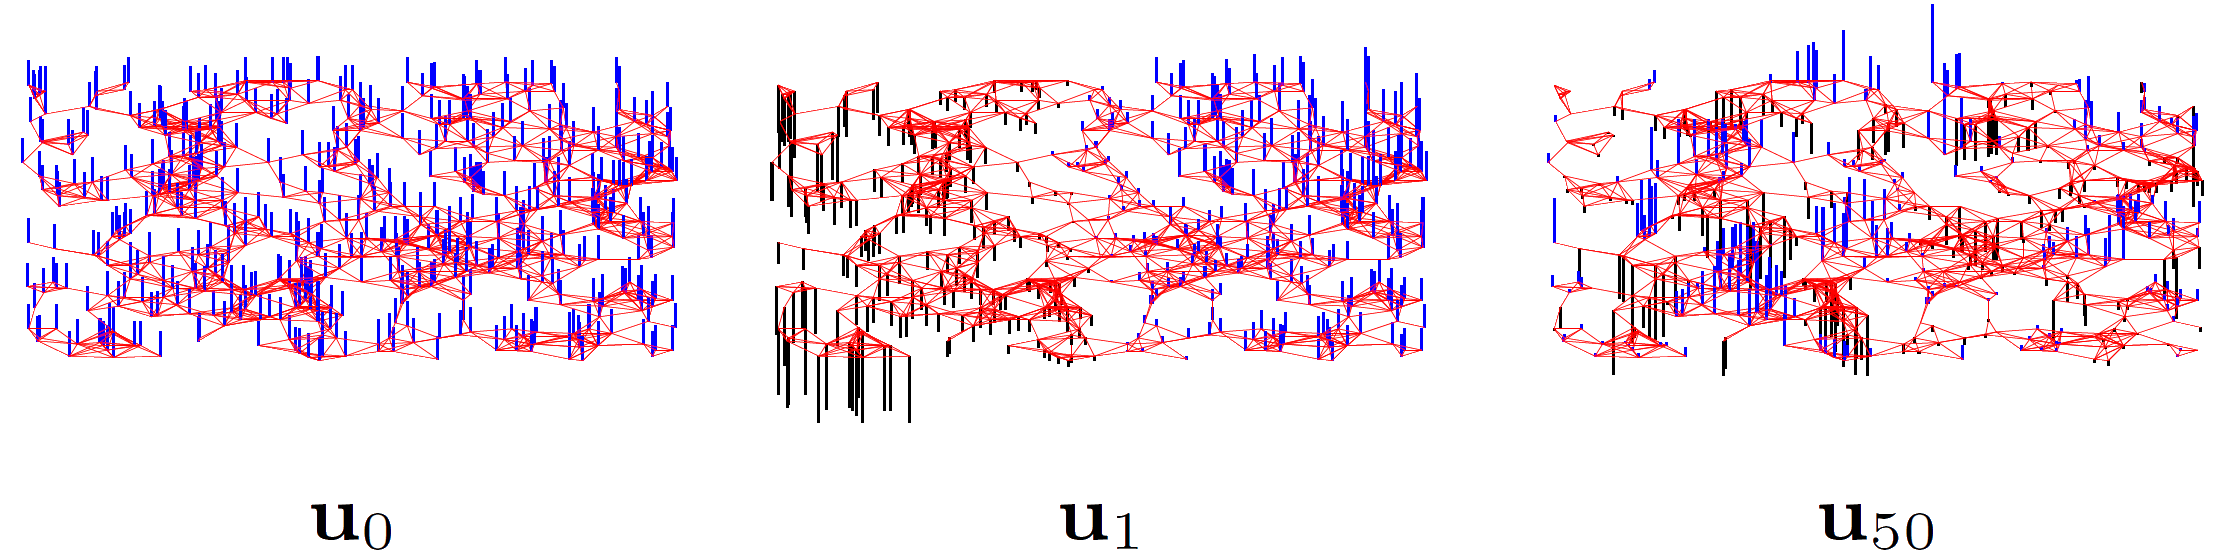
\includegraphics[width = \textwidth]{Oscillations.png}
\caption{three graph Laplacian eigenvectors for a random sensor network graph. It can be seen how $\chi_{50}$ contains definitely more zero crossing than the other two vectors $\chi_0$ and $\chi_1$}
\label{fig:osc}
\end{figure}

\subsection{Smoothness and sparsity}
In \cite{Kalofolias2016} the previous notion of smoothness is directly connected with the one of graph sparsity: in fact they show that the smoothness term can be seen equivalently as a weighted $l^1$ norm of the adjacency matrix. Minimizing this matrix can lead to a graph with a sparse set of edges that prefers only the ones associated to small distances in the \textit{pairwise distances matrix} $\Z \in \R^{N\times N}_+$ defined as $\Z_{i,j} = ||\chi_i - \chi_j||^2$.

This concept is strictly connected with the compressibility property of a signal, since previous studies validate the hypothesis that smooth signals are likely to be compressible in the frequency domain. In \cite{Zhu2012} it has been shown that the liner approximation error is upper bounded by the overall variation of the signal, this bringing to the conclusion that if the total variation of a signal is small, then the approximation error is small. This resulting in the fact that the signal can be well approximated by a small portion of the Fourier coefficients.

\section{Graph learning techniques and dictionary representation}
In \autoref{ch:introduction} we presented the main reason why signal processing field expressed the necessity of having new different structures in order to better represent the amount of information we can collect from a phenomena: what we did not focused on yet, is the fact that these amount of data are usually largely redundant, since they are a densely sampled version of the signal and they may represent multiple correlated versions of the same physical event. So normally the significative information regarding the underlying processes is largely reducible in dimensionality with respect of the collected dataset. \cite{Tosic2011} Thus, we can obtain the data representations starting from the idea that our observations can be described by a sparse subset of elementary signals - so called \textit{atoms} - taken from an \textit{overcomplete dictionary}. When the dictionary forms a basis, then every signal can be univocally represented through the linear combination of the dictionary atoms, moreover the overcompleteness property implies that atoms are linearly dependent. \cite{Tosic2011} \cite{Rubinstein2010}

With these premises, we consider a dictionary $\textbf{D} = [\textbf{d}_1, \textbf{d}_2, \dots, \textbf{d}_L] \in \R^{N \times L}$, in which the columns represent the dictionary atoms and, for the overcompleteness, $L\geq N$. Through this entity, the signal representations can be done through two main paths, either the \textit{synthesis} path, or the \textit{analysis} path, and the two can significantly differ in the overcomplete case.\\
In the synthesis path, the signal $\textbf{x} \in \R^N$ is represented as a linear combination of the dictionary atoms:
\begin{equation}
\textbf{x} = \mathcal{D}^T \gamma_s
\label{eq:synthesis}
\end{equation}
while in the analysis path it is represented through its inner product with the atoms:
\begin{equation}
\gamma_a = \mathcal{D}^T \textbf{x}
\label{eq:analysis}
\end{equation}
Where $\textbf{x}$ accounts for the sparsity concept and is called \textit{sparsity matrix}: as the name suggests, this matrix is a sparse matrix having in its columns a number of non-zero elements equal to the sparsity coefficient we impose. The sparsity coefficients indicates the number of atoms in the dictionary concurring to reproduce the signal in the vertex corresponding to the dictionary row, while the positions of these non-zeros elements in $\textbf{b}$ indicate which are the sources of this generated signal.\\

The representation in \autoref{eq:synthesis} has the consequence that, when the dictionary is overcomplete, the set of representations $\gamma_s$satisfying the equation is \textit{infinitely large}, allowing us to look for the most informative representation of the signal with respect of a certain cost function $\mathcal{C}(\gamma)$. In this way we arrive to a first general optimization problem in the form:
\begin{equation}
\gamma_s = \argmin_{\gamma} \text{  } \mathcal{C}(\gamma) \quad \text{Subject To  } \textbf{x} = \mathcal{D}\textbf{$\gamma$}
\label{eq:costF}
\end{equation}
The way we choose the form of the cost function obviously influences the structure of our solution. One of our goals is to achieve sparsity in the representation of the signal, such that the signal reconstruction is reduced in dimensionality as we are trying to achieve from the beginning. Problem stated in \autoref{eq:costF} becomes what is commonly referred as \textit{sparse coding}, and there are different functions we can apply in order to obtain it: these functions have the characteristic of being tolerant to large coefficients and, at the same time, importantly penalize small non-zero ones. Among these functions, our choice fell on the $l^1$ norm, which is one of the simplest and most effective functions of this type.

\subsection{Choosing the right dictionary}
 What we did not focused on yet is the choice of the proper dictionary for out task. In the research there has been so far, different models of dictionaries have been defined and used for the most different purposes, in the beginning the attention was mainly on traditional dictionaries, such as wavelet and Fourier dictionaries, which are simple to use and perform well for 1-dimensional signals. However, these structures were too simple to properly describe more complex and high-dimensional data, so the focus slowly moved to seeking solutions that better performed in this environment. Dictionaries emerged from this need were coming from two main sources:
 \begin{itemize}
 \item As an \textit{analytical model}, which allows to extract the dictionary straight form the data for a fast implicit implementation that does not require multiplication by the dictionary matrix;
 \item As a \textit{set of realizations} of the data, which offers an increased flexibility and adaptability to data structure;
\end{itemize}
The first model prefers speed over adaptability, since its success depends on the chosen underlying model, sometimes resulting in a over-simplistic solution for the proposed problem. From this, the necessity to also focus on the second type of dictionary, also defined as \textit{trained dictionary}.\\
Machine learning techniques of the period between 1980's and 1990's allowed to approach this problem under the new assumption that the structure of a natural phenomena can be accurately extracted \textit{straight form the data} with better results than using a mathematical formulation. The most recent training methods focus on the $l^0$ and $l^1$ sparsity measures, which have a simpler formulation and at the same time can use the more recent sparsity coding techniques. \cite{Gorodnitsky1997} \cite{Pati1993}
Among these learning methods, particular relevance acquired the \textit{parametric training methods}, such as \textit{translation-invariant dictionaries}, \textit{multiscale dictionaries} or \textit{sparse dictionaries}. These implementations involve the reduction of parameters' number and the assumption of several desirable properties on the dictionary, in the end leading to an accelerate convergence, reduced density of the local minima and the convergence to a better solution. Moreover, the generalization of the learning process is improved thanks to the smaller number of parameters, as much as the reduction in number of examples needed. Finally, parametric dictionaries bring to a more efficient implementation, due to the fact that parametrization typically has a more compact representation and, not less important, a parametric dictionary may be designed to represent infinite or arbitrary-sized signals. \cite{Rubinstein2010}

\subsubsection{The sparse approximation}
The intention of sparse approximations is to represent a certain signal $y$ of dimension $n$ as the linear combination of a small amount of signals selected from the source database, which is the dictionary. In the dictionary the elements are typically unit norm functions, called \textit{atoms}, that can be denoted through $\phi_k$ (with $k = 1,\dots, N$ and being $N$ the size of the dictionary) and span the entire space the signals live in.\\
When a dictionary is overcomplete, then every signal can be represented with the aforementioned linear combination:
\begin{equation}
\textbf{y} = \textbf{$\phi$}\textbf{a} = \sum_{k=1}^{N}a_k\phi_k
\end{equation}
and the value that \textbf{a} can assume is not unique.\\
To achieve sparse and efficient representations, the requirement for finding the exact representation is in general relaxed: starting from the NP-hard problem which is the minimization of the $l^0$ norm of \textbf{a}, we can approach the issue through convex relaxation methods that solve a problem in the form:
\begin{equation}
\min_\textbf{a} \text{ } (|| \textbf{y} - \textbf{$\phi$a} ||_2^2 + \textbf{$\lambda$}||\textbf{a}||_1)
\end{equation}
in which the relaxation allowed to replace the nonconvex $l^0$ norm in the original problem with a more meaningful $l^1$ norm. \cite{Tosic2011}

\section{Related work}
Given the premises presented in the previous sections, our work mainly focused on two open issues regarding both the dictionary learning and the graph learning problem. The starting point were the works of Dorina Thanou -  regarding the dictionary learning approach for graph signals - and the work of Hermina Petric Maretic - regarding the graph learning approach.\\
In the related work, Thanou et al. proposed a learning algorithm which was able to retrieve the kernel functions for a certain dictionary, alternatively optimizing over the kernel coefficients $\alpha$ and the sparsity matrix $X$ \cite{Thanou2014}, while Maretic et al. started from the complementary assumption that the entities known in their case where exactly the kernel coefficients, while they alternatively optimized over the sparsity matrix and the graph weight matrix \cite{Maretic2017}.

\subsection{State of the art}
There has already been a discrete amount of work around graph inference for signals that are expected to be smooth on the graph.  In \cite{Dong2016} Dong et al. addressed the problem adopting a factor analysis model for graph signals and imposing a Gaussian probabilistic prior on the independent variables which model the signal. Their results showed that smoothness property of a graph signal is favoured by the efficient representation obtained through these priors. In particular, in the algorithm they presented they deployed the use of $l^1$ and Frobenius norm, the former is expressed by a constraint on the Trace of the Laplacian, and eventually accounts for a sparsity term, while the latter is added as a penalty term in the objective function in order to control the distribution of the off-diagonal entries in L.

At the same time, in \cite{Kalofolias2016} Kalofolias proposes another framework to learn a graph structure under the smoothness assumption. They also use the minimization of the trace term for the Laplacian matrix, clinching that the minimizations of it brings to naturally sparse solutions.

However, this assumption is not always exhaustively descriptive of the real problem we are considering, so we might want to add other reinforcements to the priors in order to better describe the situation. For example, we could imagine a real world network to show a localized behavior or a more organized one having a certain pattern repeating over the graph. In \cite{Maretic2017}, this was an assumption for the signal, bringing it to be a sparse combination of a small number of atoms in a polynomial graph dictionary. This in the end was creating atoms localized in every node on the graph, repeating the same pattern over it with respect to every node as a source, in the same way it is described in \cite{Thanou2014}. However Maretic's work is limited by the fact that, as we already mentioned, it assumes the kernels to be know functions while it concentrates only on the graph dictionary and thus fixing the spectral behavior of the atoms.

\subsection{Problem structure}
As previously mentioned, this work deals with the general class of signals that can be represented in a sparse way through atoms of a polynomial dictionary \cite{Thanou2014}, such that it can give a natural segregation of each signal into localised components, as shown in \autoref{fig:components}. The figure shows how each of these components derive from one atom, which is directly dependent of the graph dictionary. This is well explained if, for polynomial kernels of degree k, we see our atoms as an entity spanning only the k-hop distance from the node that represents the center of the atom (source), as we will describe in the next section.

\begin{figure}
\centering
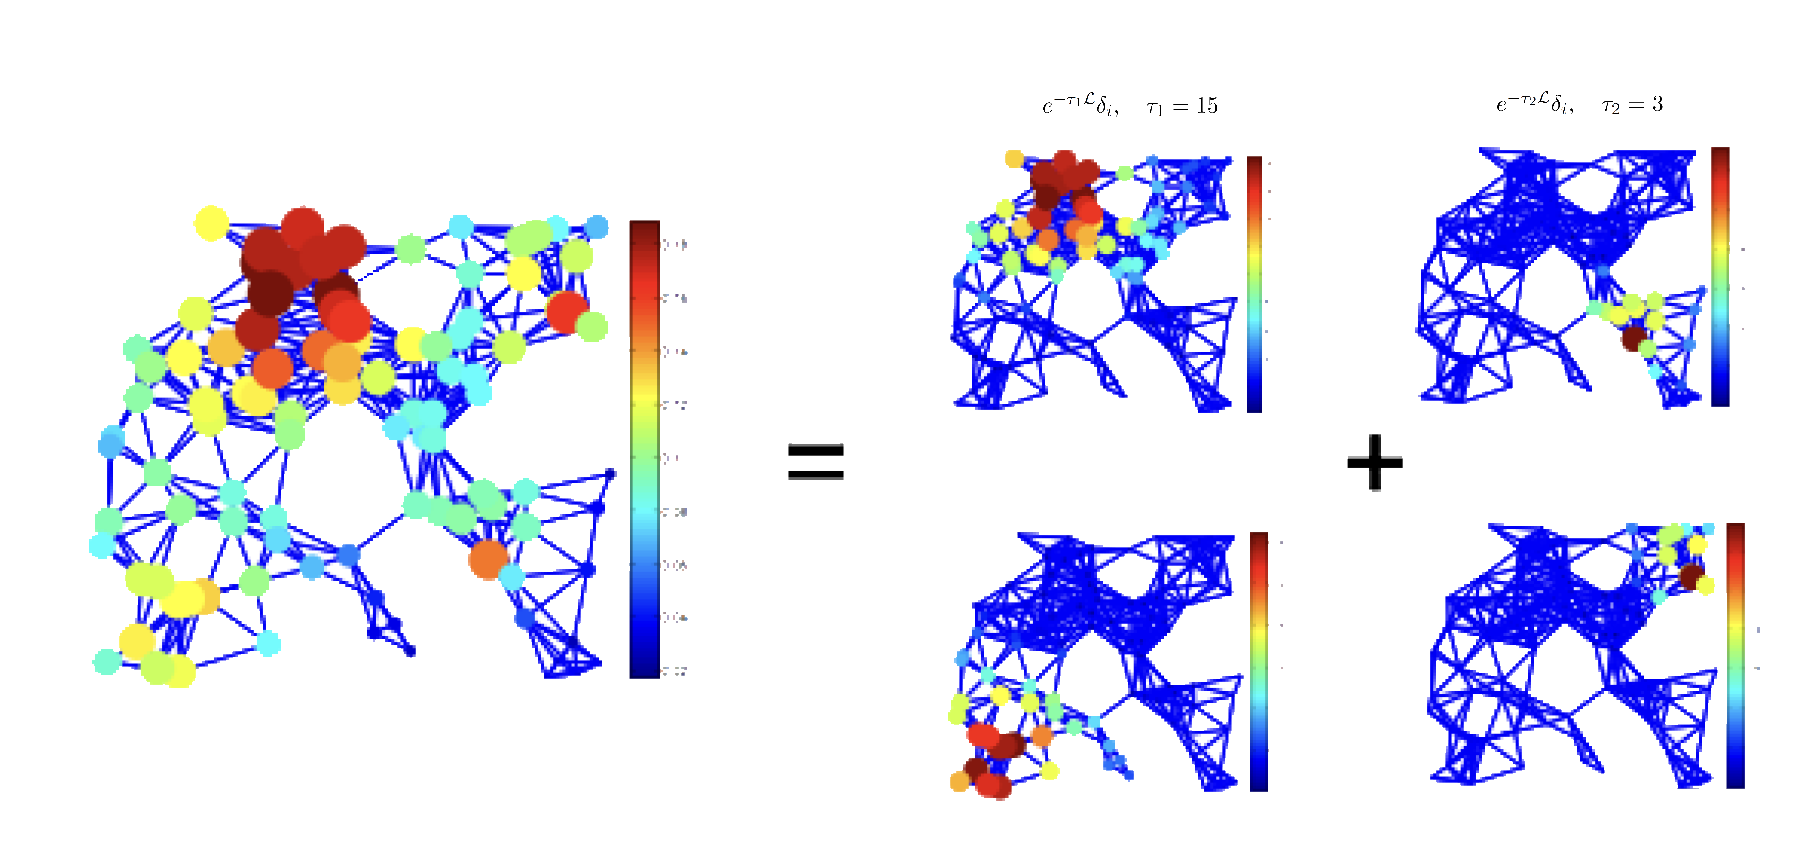
\includegraphics[width = .8\textwidth]{SignalDecomposition.png}
\caption{Example of signal decomposition using the polynomial dictionary}
\label{fig:components}
\end{figure}

In continuity with the prior work, here we assume the sources of our atoms to be unknown and not necessarily the same for all the different generated parts of the signal. This means, in mathematical terms, assuming that we do not know \textit{a priori} the position, in the columns of the sparsity matrix $X$, of the non-zero entries that indicate which are the nodes acting as sources for the atoms.

Closely related to the segregation assumption then, is the fact that we could imagine our signal as having a sort of community structure. This means that the graph can be clustered into communities that are poorly related among themselves when talking about the signal variation, thus imagining very different node signals to be sufficiently distant, and so, being part of separated communities.

% Another strictly related assumption, is that the graph has a strong community structure, meaning that the graph can be separated into communities which are poorly related among themselves, but hold strong connections inside them. These two assumptions are somewhat exchangeable, such that an interesting aspect to develop in the future could be reducing one of them.

\subsubsection{The translation operator and the smoothness priors}
To better describe the structure of our dictionary, we start recalling that in \autoref{sec:graph laplacian} we introduced the Laplacian operator as $L = D - W$ and here we focus on a modified version of this operator, that is the \textit{normalized Laplacian} $\mathcal{L} = D^{-\frac{1}{2}}LD^{-\frac{1}{2}}$. The normalized Laplacian is also a real symmetric and positive semidefinite matrix, with a complete set of orthonormal eigenvectors $\textbf{$\chi$} = [\chi_0,\chi_1,\dots,\chi_{N-1}]$ and associated non negative eigenvalues $\sigma(\mathcal{L}) := \{ 0 = \lambda_0,\lambda_1,\dots,\lambda_{N-1} \leq 2 \}$ (where the upper bound 2 comes from the normalization).
The normalized Laplacian eigenvectors are Fourier basis, this bringing any function $y$ defined on the vertices of the graph to be represented in his Fourier transform version $\hat{y}$ at frequency $\lambda_l$ as:
\begin{equation}
\hat{y}(\lambda_l) = \langle y, \chi_l \rangle = \sum_{n=1}^{N} y(n)\chi_l^{*}(n)
\end{equation}
and its relative inverse transform to be:
\begin{equation}
y(n) = \sum_{l=0}^{N-1} \hat{y}(\lambda_l)\chi_l(n), \quad \forall n \in \mathcal{V}
\end{equation}
This transform plays a major role not only in the harmonic analysis, but also in defining the signal translation onto a graph, which actually is the main transformation we are interested in when we try to construct a graph dictionary. It is worth to notice here that in the classical signal processing field the translation operator is defined through the change of variable $(T_n f)(t) := f(t-n)$, but when it comes to graph signal processing, this concept looses meaning since there is no significate to $f(\circ - n)$ in the graph environment. However, from transform theory we can recall that the classical translation operator $T_n$ can also be seen as a convolution with a Kronecker delta $\delta$ centered in $n$\cite{Shuman2013} \cite{Thanou2014}:
\begin{equation}
T_n g = \sqrt{N}(g * \delta_n) = \sqrt{N}\sum_{l=0}^{N-1}\hat{g}(\lambda_l)\chi_l^{*}(n)\chi_l \quad .
\label{eq:translation}
\end{equation}

This leads to think about \autoref{eq:translation} as an operator acting on the kernel $g(\cdot)$ directly defined in the spectral domain and from which we can obtain the effective translation to kernel $n$ through inverse graph Fourier transform. Moreover the term $\sqrt{N}$ in the \autoref{eq:translation} is a guarantee for the translation operator to preserve the mean value of the signal.\\

Now, in all of this we can assume the signal to have a smooth support as the one described in \autoref{ch:smoothness}; this prior is carried by the kernel entity  $g(\cdot)$ and can be seen as a measure to control the localization of $T_n g$ centered at vertex $n$ (meaning that the magnitude ($T_n g$)(i) of the translated kernel at vertex $i$ decays with the increasing distance from the center of the kernel). We can thus compose our atoms $T_n g$ as smooth entities, coming from the assumption that the kernel function in \autoref{eq:translation} is a smooth polynomial function of degree K:
\begin{equation}
\hat{g}(\lambda_l) = \sum_{k=0}^{K} \alpha_k\lambda_l^k, \quad l = 0,\dots,N-1
\end{equation}
From this fact, we can so obtain a global expression for a translation operator as:
\begin{align}
T_n g & = \sqrt{N}(g * \delta_n) = \sqrt{N}\sum_{l=0}^{N-1}\sum_{k=0}^{K}\alpha_k\lambda_l^k\chi_l^*(n)\chi_l \notag\\
&= \sqrt{N}\sum_{k=0}^{K}\alpha_k\sum_{l=0}^{N-1}\lambda_l^k\chi_l^*(n)\chi_l = \sqrt{N}\sum_{k=0}^{K}\alpha_k (\mathcal{L}^k)_n
\end{align}
where $(\mathcal{L})_n$ represents the $n^{th}$ column of the $k^{th}$ power of the Laplacian matrix $\mathcal{L}^k$. The final concatenation of $N$ such columns brings us to generate a set of $N$ atoms, corresponding to the columns of
\begin{equation}
Tg = \sqrt{N}\hat{g}(\mathcal{L}) = \sqrt{N}\chi \hat{g}(\Lambda)\chi^T = \sqrt{N}\sum_{k=0}^{K}\alpha_k\mathcal{L}^k
\label{eq:tg}
\end{equation}
Where the quantity $\Lambda$ corresponds to the diagonal matrix of the eigenvalues in such a way that the following relation holds: $\mathcal{L} = \rchi \Lambda \rchi^T$ \cite{Dong2016}. This brief section has the intrinsic meaning that if the kernel $g(\cdot)$ is a polynomial of degree $K$, then the translation operator is $0$ in all the vertices $i$ that are more than $K$ hops far away from the center vertex $n$, which means that the vertex domain support of the translated vertex is contained in a sphere of radius $K$ and center in $n$ and its magnitude decades with the increasing distance from $n$ to $i$.
In \autoref{fig:minnesota} there is an example of an atom translation in three different ways.

\begin{figure}[tb]
  \centering
  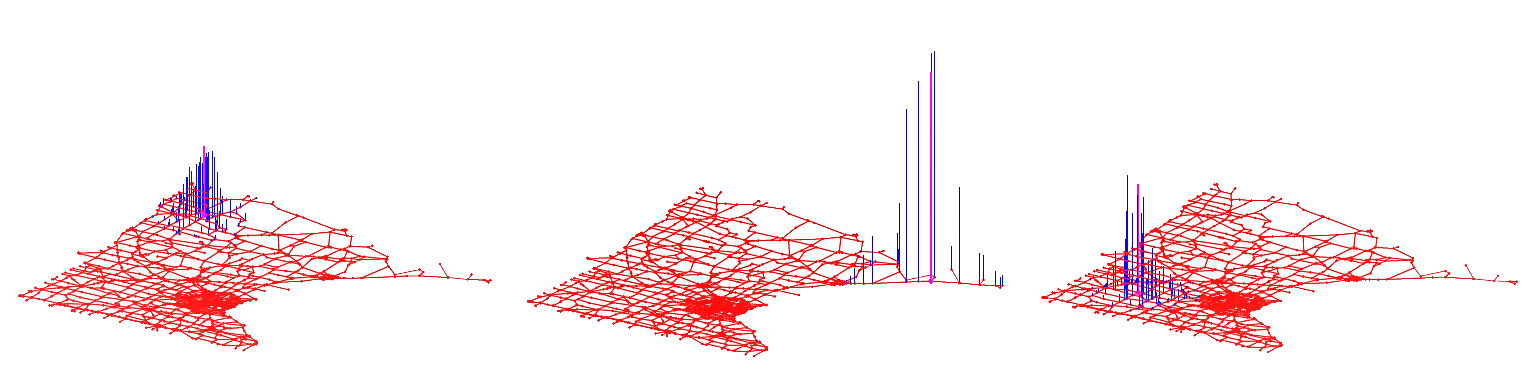
\includegraphics[width = \textwidth]{MinnesotaTranslation.png}
  \caption{Example of graph signal translation: translation for $T_{200}g$ (a), $T_{1000}g$ (b) and $T_{2000}g$ (c)}
  \label{fig:minnesota}
\end{figure}
